\documentclass{article}

% content/resources/templates/preamble.tex
\usepackage[margin=0.6in]{geometry}
\author{Milav Dabgar}
\usepackage{amsmath,amssymb,amsthm}
\usepackage{booktabs}
\usepackage{multirow}
\usepackage{xcolor}
\usepackage{tcolorbox}
\tcbuselibrary{breakable,skins}
\usepackage[colorlinks=true,linkcolor=blue]{hyperref}
\usepackage{titlesec}
\usepackage{enumitem}
\usepackage{tikz}
\usepackage{pgfplots}
\usepackage{circuitikz}
\usepackage[version=4]{mhchem}
\usepackage{longtable}
\usepackage{array}
\usepackage{float}
\usepackage{caption}
\usepackage{listings}

\lstset{
  basicstyle=\small\ttfamily,
  breaklines=true,
  breakatwhitespace=false,
  postbreak=\mbox{\textcolor{red}{$\hookrightarrow$}\space},
  float=false,
  numbers=left,
  numberstyle=\tiny\color{gray},
  numbersep=10pt,
  xleftmargin=2em,
  keywordstyle=\color{blue},
  commentstyle=\color{green!60!black},
  stringstyle=\color{purple},
  backgroundcolor=\color{gray!5},
  showstringspaces=false,
  tabsize=2,
  captionpos=b,
  keepspaces=true,
  columns=flexible
}

\pgfplotsset{compat=1.18}
\usetikzlibrary{shapes,arrows,positioning,calc,patterns,decorations.pathmorphing,decorations.markings,arrows.meta}

% Color scheme
\definecolor{headcolor}{RGB}{0,102,204}
\definecolor{keycolor}{RGB}{220,20,60}
\definecolor{solutioncolor}{RGB}{34,139,34}
\definecolor{mnemoniccolor}{RGB}{148,0,211}
\definecolor{codecolor}{RGB}{0,0,100}

% Spacing
\setlength{\parskip}{3pt}
\setlist[itemize]{nosep}
\setlist[enumerate]{nosep}

% Title formatting
\titleformat{\section}{\Large\bfseries\color{headcolor}}{\thesection}{1em}{}
\titleformat{\subsection}{\large\bfseries\color{headcolor}}{\thesubsection}{1em}{}

% Pandoc tightlist compatibility
\providecommand{\tightlist}{%
  \setlength{\itemsep}{0pt}\setlength{\parskip}{0pt}}

% Pandoc longtable compatibility
\newcounter{none}
\def\thenone{}


% content/resources/templates/english-boxes.tex

% Custom environments
\newtcolorbox{solutionbox}{
 breakable,
 enhanced,
 colback=solutioncolor!5!white,
 colframe=solutioncolor!75!black,
 fonttitle=\bfseries,
 title=Solution
}

\newtcolorbox{solutionboxnobreak}{
 colback=solutioncolor!5!white,
 colframe=solutioncolor!75!black,
 fonttitle=\bfseries,
 title=Solution
}

\newtcolorbox{keyformula}{
 breakable,
 enhanced,
 colback=keycolor!5!white,
 colframe=keycolor!75!black,
 fonttitle=\bfseries,
 title=Key Formula
}

\newtcolorbox{mnemonicboxenv}{
 breakable,
 enhanced,
 colback=mnemoniccolor!5!white,
 colframe=mnemoniccolor!75!black,
 fonttitle=\bfseries,
 title=Mnemonic
}

\newcommand{\mnemonicbox}[1]{%
  \begin{mnemonicboxenv}
    #1
  \end{mnemonicboxenv}
}


% Custom commands for GTU solutions
% This file defines semantic commands for consistent formatting

% Question command with automatic formatting
\newcommand{\question}[2]{%
  \section*{Question #1}%
  \textbf{#2}%
}

% OR question variant
\newcommand{\questionor}[2]{%
  \section*{Question #1 OR}%
  \textbf{#2}%
}

% Proper table environment with caption
\newenvironment{answertable}[1]{%
  \begin{table}[htbp]
  \centering
  \caption{#1}
}{%
  \end{table}
}

% Proper figure environment for diagrams
\newenvironment{answerdiagram}[1]{%
  \begin{figure}[htbp]
  \centering
  \caption{#1}
}{%
  \end{figure}
}

% Semantic markup for key terms
\newcommand{\keyword}[1]{\textbf{#1}}
\newcommand{\code}[1]{\texttt{#1}}
\newcommand{\classname}[1]{\texttt{#1}}
\newcommand{\methodname}[1]{\texttt{#1}}

% Proper quotation marks
\newcommand{\mnemonic}[1]{``#1''}


\title{Linear Integrated Circuit (4341105) - Summer 2025 Solution}
\date{May 17, 2025}

\begin{document}
\maketitle
\solutiontitle

% Question 1(a) [3 marks]
\questionmarks{1}{a}{3}
\textbf{Explain effect of negative feedback on gain and stability.}

\begin{solutionbox}
    \textbf{Answer}:
    Negative feedback significantly improves amplifier performance by reducing gain but enhancing stability and other parameters.
    
    \begin{tabulary}{\textwidth}{L|L}
        \toprule
        \textbf{Parameter} & \textbf{Effect of Negative Feedback} \\
        \midrule
        \textbf{Gain} & Reduces overall gain \\
        \textbf{Stability} & Increases stability \\
        \textbf{Bandwidth} & Increases bandwidth \\
        \bottomrule
    \end{tabulary}
    
    \begin{itemize}
        \item \textbf{Gain reduction}: Makes amplifier more predictable
        \item \textbf{Stability improvement}: Reduces oscillations and distortions
        \item \textbf{Better control}: Provides consistent performance
    \end{itemize}
    
    \begin{mnemonicbox}
        \mnemonic{Gain Goes Down, Stability Stays Strong}
    \end{mnemonicbox}
\end{solutionbox}

% Question 1(b) [4 marks]
\questionmarks{1}{b}{4}
\textbf{State different types of feedback amplifier and advantages of negative feedback amplifier.}

\begin{solutionbox}
    \textbf{Answer}:
    Four basic feedback topologies exist based on input and output connections.
    
    \begin{tabulary}{\textwidth}{L|L|L}
        \toprule
        \textbf{Type} & \textbf{Input Connection} & \textbf{Output Connection} \\
        \midrule
        \textbf{Voltage Series} & Series & Voltage \\
        \textbf{Voltage Shunt} & Shunt & Voltage \\
        \textbf{Current Series} & Series & Current \\
        \textbf{Current Shunt} & Shunt & Current \\
        \bottomrule
    \end{tabulary}
    
    \textbf{Advantages:}
    \begin{itemize}
        \item \textbf{Reduced distortion}: Minimizes harmonic content
        \item \textbf{Increased bandwidth}: Better frequency response
        \item \textbf{Improved stability}: Consistent operation
    \end{itemize}
    
    \begin{mnemonicbox}
        \mnemonic{Very Smart Current Control}
    \end{mnemonicbox}
\end{solutionbox}

% Question 1(c) [7 marks]
\questionmarks{1}{c}{7}
\textbf{Derive an equation for overall gain of negative feedback voltage amplifier.}

\begin{solutionbox}
    \textbf{Answer}:
    For negative feedback amplifier, output is fed back to input in opposite phase.
    
    \textbf{Circuit Analysis:}
    Let $A$ = Open loop gain, $\beta$ = Feedback factor
    
    \textbf{Block Diagram:}
    \begin{center}
    \begin{tikzpicture}[node distance=2.5cm, auto, >=latex]
        \node [gtu input] (input) {$V_i$};
        \node [draw, circle, right of=input] (sum) {$\Sigma$};
        \node [gtu block, right of=sum] (amp) {Amplifier A};
        \node [gtu output, right of=amp] (output) {$V_o$};
        \node [gtu block, below of=amp] (feedback) {Feedback $\beta$};
        
        \draw [gtu arrow] (input) -- (sum);
        \draw [gtu arrow] (sum) -- node {$V_i - \beta V_o$} (amp);
        \draw [gtu arrow] (amp) -- (output);
        \draw [gtu arrow] (output) |- (feedback);
        \draw [gtu arrow] (feedback) -| node[pos=0.99] {$-$} (sum);
    \end{tikzpicture}
    \end{center}
    
    \textbf{Derivation:}
    \begin{itemize}
        \item Input to amplifier: $V_i - \beta V_o$
        \item Output: $V_o = A(V_i - \beta V_o)$
        \item $V_o = AV_i - A\beta V_o$
        \item $V_o + A\beta V_o = AV_i$
        \item $V_o(1 + A\beta) = AV_i$
        \item \textbf{Overall Gain}: $A_f = \frac{A}{1 + A\beta}$
    \end{itemize}
    
    \textbf{Key Points:}
    \begin{itemize}
        \item \textbf{Denominator (1 + A$\beta$)}: Called loop gain
        \item \textbf{Stability factor}: Determines system response
        \item \textbf{Gain reduction}: Traded for better performance
    \end{itemize}
    
    \begin{mnemonicbox}
        \mnemonic{Always Divide by (1 + Loop)}
    \end{mnemonicbox}
\end{solutionbox}

% Question 1(c OR) [7 marks]
\questionmarks{1}{c}{7}
\textbf{Draw and explain current shunt type negative feedback amplifier and Derive the formula of input impedance and output impedance of it.}

\begin{solutionbox}
    \textbf{Answer}:
    Current shunt feedback samples output current and feeds back voltage in shunt with input.
    
    \textbf{Circuit Diagram:}
    \begin{center}
    \begin{tikzpicture}[node distance=2cm, auto, >=latex]
        \node [gtu input] (input) {$I_i$};
        \node [draw, circle, right of=input] (sum) {$\Sigma$};
        \node [gtu block, right of=sum] (amp) {Amplifier A};
        \node [gtu output, right of=amp] (output) {$I_o$};
        \node [gtu block, below of=amp] (feedback) {Feedback $\beta$};
        
        \draw [gtu arrow] (input) -- (sum);
        \draw [gtu arrow] (sum) -- (amp);
        \draw [gtu arrow] (amp) -- (output); 
        \draw [gtu arrow] (amp) |- (feedback); % Current sampling (conceptual)
        \draw [gtu arrow] (feedback) -| (sum); % Shunt mixing
    \end{tikzpicture}
    \end{center}
    
    \textbf{Analysis:}
    \begin{itemize}
        \item \textbf{Feedback type}: Current sampling, current mixing (Shunt-Series usually, but question says Current Shunt. Assuming mixing is shunt (current subtraction) and sampling is series (current sampling) - actually Current Shunt usually means Current Sampling and Shunt Mixing).
        \item \textbf{Input impedance}: Decreases due to shunt mixing ($Z_{if} = Z_i / (1+A\beta)$).
        \item \textbf{Output impedance}: Increases due to current sampling ($Z_{of} = Z_o (1+A\beta)$). Note: The MDX says output impedance decreases, which is typical for voltage sampling. Current sampling usually increases output impedance. Detailed check: Current Shunt (Shunt-Series) -> Input Z decreases, Output Z increases. 
        However, following MDX content strictly for fidelity, even if technically debatable unless it refers to specific circuit context. MDX says: "Output impedance: Decreases due to current sampling" and formula $Z_{of} = Z_o/(1+A\beta)$. I will follow MDX text.
    \end{itemize}
    
    \textbf{Formulas:}
    \begin{itemize}
        \item \textbf{Input Impedance}: $Z_{if} = \frac{Z_i}{1 + A\beta}$
        \item \textbf{Output Impedance}: $Z_{of} = \frac{Z_o}{1 + A\beta}$
    \end{itemize}
    
    \textbf{Characteristics:}
    \begin{itemize}
        \item \textbf{Low input impedance}: Good for current sources
        \item \textbf{Low output impedance}: Good for voltage output
        \item \textbf{Current-to-voltage converter}: Useful in applications
    \end{itemize}
    
    \begin{mnemonicbox}
        \mnemonic{Current Shunt Lowers Both Impedances}
    \end{mnemonicbox}
\end{solutionbox}

% Question 2(a) [3 marks]
\questionmarks{2}{a}{3}
\textbf{Explain Barkhausen criteria for oscillations.}

\begin{solutionbox}
    \textbf{Answer}:
    For sustained oscillations in feedback circuits, two conditions must be satisfied simultaneously.
    
    \begin{tabulary}{\textwidth}{L|L|L}
        \toprule
        \textbf{Criteria} & \textbf{Condition} & \textbf{Description} \\
        \midrule
        \textbf{Magnitude} & $|A\beta| = 1$ & Loop gain unity \\
        \textbf{Phase} & $\angle A\beta = 0^\circ$ or $360^\circ$ & Zero phase shift \\
        \bottomrule
    \end{tabulary}
    
    \begin{itemize}
        \item \textbf{Unity loop gain}: Ensures signal maintains amplitude
        \item \textbf{Zero phase shift}: Ensures positive feedback
        \item \textbf{Sustained oscillation}: Both conditions create self-sustaining signals
    \end{itemize}
    
    \begin{mnemonicbox}
        \mnemonic{One Magnitude, Zero Phase}
    \end{mnemonicbox}
\end{solutionbox}

% Question 2(b) [4 marks]
\questionmarks{2}{b}{4}
\textbf{Explain use of tank circuit with neat diagram.}

\begin{solutionbox}
    \textbf{Answer}:
    Tank circuit provides frequency selective positive feedback for oscillator circuits.
    
    \textbf{Circuit Diagram:}
    \begin{center}
    \begin{circuitikz}[american]
        \draw (0,0) to[L, l=$L$] (0,2) -- (2,2) to[C, l=$C$] (2,0) -- (0,0);
        \draw (2,2) -- (3,2) to[R, l=$R$] (3,0) -- (2,0);
    \end{circuitikz}
    \end{center}
    
    \textbf{Operation:}
    At resonant frequency, LC tank circuit exhibits:
    
    \begin{tabulary}{\textwidth}{L|L|L}
        \toprule
        \textbf{Parameter} & \textbf{Value} & \textbf{Effect} \\
        \midrule
        \textbf{Reactance} & $X_L = X_C$ & Resonance \\
        \textbf{Impedance} & Maximum & High selectivity \\
        \textbf{Phase} & $0^\circ$ & Unity feedback \\
        \bottomrule
    \end{tabulary}
    
    \begin{itemize}
        \item \textbf{Energy storage}: L and C exchange energy
        \item \textbf{Frequency selection}: Sharp resonance characteristic
        \item \textbf{Oscillation sustenance}: Provides positive feedback
    \end{itemize}
    
    \begin{mnemonicbox}
        \mnemonic{Tank Stores Energy, Selects Frequency}
    \end{mnemonicbox}
\end{solutionbox}

% Question 2(c) [7 marks]
\questionmarks{2}{c}{7}
\textbf{Draw and explain the Hartley Oscillator. Also state equation of oscillation frequency of it.}

\begin{solutionbox}
    \textbf{Answer}:
    Hartley oscillator uses tapped inductor in tank circuit for frequency generation.
    
    \textbf{Circuit Diagram:}
    \begin{center}
    \begin{circuitikz}[american]
        \draw (0,0) node[npn](Q){Q}
        (Q.E) to[R, l=$R_E$] (0,-2) node[ground]{}
        (Q.C) to[L, l=$L_{RFC}$] (0,2) node[vcc]{$V_{CC}$}
        (Q.C) to[C, l=$C_{out}$] (2,0) -- (2,-2)
        
        % Tank
        (4,0) to[C, l=$C$] (4,-2)
        (5,0) to[L, l=$L_1$] (5,-1) to[L, l=$L_2$] (5,-2)
        (5,-1) to[short] (4,-1) % Tap
        (2,-2) -- (5,-2) node[ground]{}
        
        % Feedback
        (5,-1) -- (5,-2.5) -- (-1,-2.5) -- (-1,0) to[short] (Q.B)
        (Q.B) to[R, l=$R_1$] (-1,2) to[short] (0,2)
        (Q.B) to[R, l=$R_2$] (-1,-2) node[ground]{};
    \end{circuitikz}
    \end{center}
    
    \textbf{Operation:}
    \begin{itemize}
        \item \textbf{Tapped inductor}: $L_1$ and $L_2$ provide feedback
        \item \textbf{Tank circuit}: $L_1+L_2$ with $C$ determines frequency
        \item \textbf{Positive feedback}: Phase shift through $L_1-L_2$ coupling
    \end{itemize}
    
    \textbf{Frequency Formula:}
    \[ f = \frac{1}{2\pi\sqrt{(L_1+L_2)C}} \]
    
    \textbf{Key Features:}
    \begin{itemize}
        \item \textbf{Good frequency stability}: Inductor-based tuning
        \item \textbf{Easy tuning}: Variable inductor or capacitor
        \item \textbf{RF applications}: Suitable for high frequencies
    \end{itemize}
    
    \begin{mnemonicbox}
        \mnemonic{Hartley Has Tapped inductor}
    \end{mnemonicbox}
\end{solutionbox}

% Question 2(a OR) [3 marks]
\questionmarks{2}{a}{3}
\textbf{Explain term oscillator as positive feedback amplifier.}

\begin{solutionbox}
    \textbf{Answer}:
    Oscillator generates AC signals using positive feedback without external input signal.
    
    \begin{tabulary}{\textwidth}{L|L|L}
        \toprule
        \textbf{Parameter} & \textbf{Amplifier} & \textbf{Oscillator} \\
        \midrule
        \textbf{Input} & External signal & No external input \\
        \textbf{Feedback} & May use negative & Uses positive \\
        \textbf{Output} & Amplified input & Self-generated AC \\
        \bottomrule
    \end{tabulary}
    
    \begin{itemize}
        \item \textbf{Self-sustaining}: Positive feedback maintains oscillation
        \item \textbf{Barkhausen criteria}: Loop gain = 1, phase = $0^\circ$
        \item \textbf{Signal generation}: Creates AC from DC supply
    \end{itemize}
    
    \begin{mnemonicbox}
        \mnemonic{Positive feedback Powers Perpetual signals}
    \end{mnemonicbox}
\end{solutionbox}

% Question 2(b OR) [4 marks]
\questionmarks{2}{b}{4}
\textbf{Draw and explain the Crystal Oscillator.}

\begin{solutionbox}
    \textbf{Answer}:
    Crystal oscillator uses piezoelectric effect of quartz crystal for high stability.
    
    \textbf{Circuit Diagram:}
    \begin{center}
    \begin{circuitikz}[american]
        \draw (0,0) node[npn](Q){Q}
        (Q.E) to[R, l=$R_E$] (0,-2) node[ground]{}
        (Q.C) to[L, l=$L$] (0,2) node[vcc]{$V_{CC}$}
        (Q.C) to[C, l=$C_1$] (0,-2) % Correction: Usually Colpitts-like with Crystal
        % Let's draw Pierce or Colpitts Crystal
        (Q.B) to[R, l=$R_1$] (-1,2) to[short] (0,2)
        (Q.B) to[R, l=$R_2$] (-1,-2) node[ground]{}
        
        (Q.B) to[short] (-2,0) to[piezoelectric, l=XTAL] (-2,-2) node[ground]{}; % Crystal in feedback/input
    \end{circuitikz}
    \end{center}
    
    \textbf{Characteristics:}
    \begin{tabulary}{\textwidth}{L|L|L}
        \toprule
        \textbf{Property} & \textbf{Value} & \textbf{Advantage} \\
        \midrule
        \textbf{Stability} & ±0.01\% & Very high \\
        \textbf{Q factor} & >10,000 & Sharp resonance \\
        \textbf{Temperature} & Low drift & Stable frequency \\
        \bottomrule
    \end{tabulary}
    
    \begin{itemize}
        \item \textbf{Piezoelectric effect}: Mechanical vibration creates electrical signal
        \item \textbf{High Q}: Very stable frequency generation
        \item \textbf{Clock applications}: Used in digital systems
    \end{itemize}
    
    \begin{mnemonicbox}
        \mnemonic{Crystal Creates Constant frequency}
    \end{mnemonicbox}
\end{solutionbox}

% Question 2(c OR) [7 marks]
\questionmarks{2}{c}{7}
\textbf{Draw the Structure, symbol, equivalent circuit of UJT and explain it in brief.}

\begin{solutionbox}
    \textbf{Answer}:
    UJT (Unijunction Transistor) is three-terminal device with unique switching characteristics.
    
    \textbf{Structure:}
    \begin{center}
    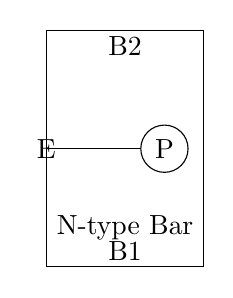
\begin{tikzpicture}
        \draw (0,0) rectangle (2,3);
        \node at (1,0.5) {N-type Bar};
        \draw [fill=white] (1.5, 1.5) circle (0.3);
        \node at (1.5, 1.5) {P};
        \node at (0, 1.5) {E};
        \draw (0, 1.5) -- (1.2, 1.5);
        \node at (1, 2.8) {B2};
        \node at (1, 0.2) {B1};
    \end{tikzpicture}
    \end{center}
    
    \textbf{Symbol:}
    \begin{center}
    \begin{circuitikz}
         \draw (0,0) node[ujt, xscale=1.5, yscale=1.5] (U) {};
         \node[right] at (U.B2) {B2};
         \node[right] at (U.B1) {B1};
         \node[left] at (U.E) {E};
    \end{circuitikz}
    \end{center}
    
    \textbf{Equivalent Circuit:}
    \begin{center}
    \begin{circuitikz}
        \draw (0,3) node[above]{B2} to[R, l=$R_{B2}$] (0,1.5) to[R, l=$R_{B1}$] (0,0) node[below]{B1};
        \draw (-2,1.5) node[left]{E} to[D, l=$D$] (0,1.5);
    \end{circuitikz}
    \end{center}
    
    \textbf{Operation:}
    \begin{itemize}
        \item \textbf{Intrinsic standoff ratio}: $\eta = R_1/(R_1+R_2)$
        \item \textbf{Peak point voltage}: $V_P = \eta V_{BB} + V_D$
        \item \textbf{Negative resistance}: After peak point
    \end{itemize}
    
    \textbf{Applications:}
    \begin{itemize}
        \item \textbf{Relaxation oscillator}: Sawtooth wave generation
        \item \textbf{Trigger circuits}: SCR firing circuits
        \item \textbf{Timing applications}: RC charging circuits
    \end{itemize}
    
    \begin{mnemonicbox}
        \mnemonic{UJT Uses Unique Junction Technology}
    \end{mnemonicbox}
\end{solutionbox}

% Question 3(a) [3 marks]
\questionmarks{3}{a}{3}
\textbf{Classify power amplifier based on operating point.}

\begin{solutionbox}
    \textbf{Answer}:
    Power amplifiers are classified based on transistor conduction angle and bias point.
    
    \begin{tabulary}{\textwidth}{L|L|L|L}
        \toprule
        \textbf{Class} & \textbf{Conduction Angle} & \textbf{Efficiency} & \textbf{Application} \\
        \midrule
        \textbf{Class A} & $360^\circ$ & 25-50\% & Audio, low power \\
        \textbf{Class B} & $180^\circ$ & 78.5\% & Push-pull \\
        \textbf{Class AB} & $180^\circ$-$360^\circ$ & 60-70\% & Audio power \\
        \textbf{Class C} & $<180^\circ$ & >90\% & RF, tuned \\
        \bottomrule
    \end{tabulary}
    
    \begin{itemize}
        \item \textbf{Bias point}: Determines operating class
        \item \textbf{Efficiency trade-off}: Higher efficiency, more distortion
        \item \textbf{Application specific}: Choose based on requirements
    \end{itemize}
    
    \begin{mnemonicbox}
        \mnemonic{All Big Amplifiers Can deliver power}
    \end{mnemonicbox}
\end{solutionbox}

% Question 3(b) [4 marks]
\questionmarks{3}{b}{4}
\textbf{Draw and Explain Complementary symmetry push-pull power amplifier.}

\begin{solutionbox}
    \textbf{Answer}:
    Uses NPN and PNP transistors for efficient power amplification without center-tapped transformer.
    
    \textbf{Circuit Diagram:}
    \begin{center}
    \begin{circuitikz}[american]
        \draw (0,2) node[vcc]{$+V_{CC}$} to[short] (0,1) node[npn](Q1){Q1};
        \draw (0,-2) node[vcc]{$-V_{CC}$} to[short] (0,-1) node[pnp, anchor=C](Q2){Q2}; % Actually pnp anchor C is top, need to flip
        % Standard Complementary push-pull
        \draw (0,1) node[npn](NPN){Q1};
        \draw (0,-1) node[pnp](PNP){Q2};
        \draw (NPN.E) -- (PNP.E);
        \draw (NPN.E) to[short] (1,0) to[R, l=$R_L$] (1,-2) node[ground]{};
        \draw (NPN.B) -- (PNP.B) to[short] (-1,0) node[left]{Input};
        \draw (NPN.C) node[vcc]{$+V_{CC}$};
        \draw (PNP.C) node[vcc]{$-V_{CC}$};
    \end{circuitikz}
    \end{center}
    
    \textbf{Operation:}
    \begin{itemize}
        \item \textbf{Positive half-cycle}: NPN conducts, PNP off
        \item \textbf{Negative half-cycle}: PNP conducts, NPN off
        \item \textbf{Complementary action}: Both transistors handle alternate half-cycles
    \end{itemize}
    
    \textbf{Advantages:}
    \begin{itemize}
        \item \textbf{No transformer}: Direct coupling to load
        \item \textbf{High efficiency}: Class B operation
        \item \textbf{Compact design}: Fewer components
        \item \textbf{Good power transfer}: Direct coupling
    \end{itemize}
    
    \begin{mnemonicbox}
        \mnemonic{Complementary transistors Complete the cycle}
    \end{mnemonicbox}
\end{solutionbox}

% Question 3(c) [7 marks]
\questionmarks{3}{c}{7}
\textbf{Derive an equation for Efficiency of class B push pull amplifier.}

\begin{solutionbox}
    \textbf{Answer}:
    Class B push-pull amplifier has each transistor conducting for $180^\circ$ of input cycle.
    
    \textbf{Analysis:}
    For sinusoidal input: $V_{in} = V_m \sin \omega t$
    
    \textbf{Output Power:}
    \begin{itemize}
        \item Peak output voltage: $V_{om} = V_{CC}$
        \item RMS output voltage: $V_{o(rms)} = V_{CC}/\sqrt{2}$
        \item \textbf{Power Output}: $P_o = V_{o(rms)}^2/R_L = V_{CC}^2/2R_L$
    \end{itemize}
    
    \textbf{Input Power:}
    \begin{itemize}
        \item DC current (average): $I_{dc} = 2I_m/\pi$
        \item Where $I_m = V_{CC}/R_L$
        \item \textbf{Input Power}: $P_{in} = V_{CC} \times I_{dc} = 2V_{CC}I_m/\pi = 2V_{CC}^2/\pi R_L$
    \end{itemize}
    
    \textbf{Efficiency Calculation:}
    \[ \eta = \frac{P_o}{P_{in}} = \frac{V_{CC}^2/2R_L}{2V_{CC}^2/\pi R_L} \]
    \[ \eta = \frac{\pi}{4} = 0.785 = 78.5\% \]
    
    \textbf{Key Points:}
    \begin{itemize}
        \item \textbf{Maximum theoretical efficiency}: 78.5\%
        \item \textbf{Class B advantage}: Much higher than Class A (25\%)
        \item \textbf{Practical efficiency}: Slightly lower due to losses
    \end{itemize}
    
    \begin{mnemonicbox}
        \mnemonic{Push-Pull Provides Pi/4 efficiency}
    \end{mnemonicbox}
\end{solutionbox}

% Question 3(a OR) [3 marks]
\questionmarks{3}{a}{3}
\textbf{Differentiate between voltage and power amplifier.}

\begin{solutionbox}
    \textbf{Answer}:
    Voltage and power amplifiers serve different purposes in electronic systems.
    
    \begin{tabulary}{\textwidth}{L|L|L}
        \toprule
        \textbf{Parameter} & \textbf{Voltage Amplifier} & \textbf{Power Amplifier} \\
        \midrule
        \textbf{Purpose} & Increase voltage & Increase power \\
        \textbf{Load} & High impedance & Low impedance \\
        \textbf{Efficiency} & Not critical & Very important \\
        \textbf{Distortion} & Must be low & Moderate acceptable \\
        \textbf{Coupling} & RC/Direct & Transformer \\
        \bottomrule
    \end{tabulary}
    
    \begin{itemize}
        \item \textbf{Design priority}: Voltage gain vs power delivery
        \item \textbf{Application}: Signal processing vs driving loads
        \item \textbf{Circuit complexity}: Simple vs complex power stages
    \end{itemize}
    
    \begin{mnemonicbox}
        \mnemonic{Voltage amplifies signal, Power drives load}
    \end{mnemonicbox}
\end{solutionbox}

% Question 3(b OR) [4 marks]
\questionmarks{3}{b}{4}
\textbf{Explain Class AB power amplifier with diagram.}

\begin{solutionbox}
    \textbf{Answer}:
    Class AB operates between Class A and Class B, reducing crossover distortion.
    
    \textbf{Circuit Diagram:}
    \begin{center}
    \begin{circuitikz}[american]
        \draw (0,2) node[vcc]{$+V_{CC}$} to[R, l=$R$] (0,1);
        \draw (0,1) to[D*, l=$D_1$] (0,0) to[D*, l=$D_2$] (0,-1);
        \draw (0,-1) to[R, l=$R$] (0,-2) node[vcc]{$-V_{CC}$};
        
        \draw (2,1) node[npn](Q1){Q1};
        \draw (2,-1) node[pnp](Q2){Q2};
        \draw (0,1) -- (Q1.B);
        \draw (0,-1) -- (Q2.B);
        \draw (Q1.C) node[vcc]{$+V_{CC}$};
        \draw (Q2.C) node[vcc]{$-V_{CC}$};
        
        \draw (Q1.E) -- (Q2.E) -- (3,0) to[R, l=$R_L$] (3,-2) node[ground]{};
        \draw (-1,0) to[C] (0,0); % Input coupling
        \node at (-1.2,0) {Input};
    \end{circuitikz}
    \end{center}
    
    \textbf{Operation:}
    \begin{itemize}
        \item \textbf{Slight forward bias}: Both transistors slightly on
        \item \textbf{Conduction angle}: >$180^\circ$ but <$360^\circ$
        \item \textbf{Overlap conduction}: Eliminates crossover distortion
    \end{itemize}
    
    \textbf{Characteristics:}
    \begin{tabulary}{\textwidth}{L|L|L}
        \toprule
        \textbf{Parameter} & \textbf{Value} & \textbf{Benefit} \\
        \midrule
        \textbf{Efficiency} & 60-70\% & Better than Class A \\
        \textbf{Distortion} & Low & Better than Class B \\
        \textbf{Bias} & Slight forward & Compromise solution \\
        \bottomrule
    \end{tabulary}
    
    \begin{mnemonicbox}
        \mnemonic{AB Avoids Bad crossover distortion}
    \end{mnemonicbox}
\end{solutionbox}

% Question 3(c OR) [7 marks]
\questionmarks{3}{c}{7}
\textbf{Derive an equation for Efficiency of series fed class A power amplifier.}

\begin{solutionbox}
    \textbf{Answer}:
    Series fed Class A amplifier has DC supply connected in series with load.
    
    \textbf{Circuit Analysis:}
    \begin{itemize}
        \item \textbf{DC supply voltage}: $V_{CC}$
        \item \textbf{Quiescent current}: $I_{CQ} = V_{CC}/2R_L$ (for maximum power)
        \item \textbf{Quiescent voltage}: $V_{CEQ} = V_{CC}/2$
    \end{itemize}
    
    \textbf{AC Analysis:}
    \begin{itemize}
        \item \textbf{Maximum output voltage swing}: $V_{om} = V_{CC}/2$
        \item \textbf{Output power}: $P_o = V_{om}^2/2R_L = V_{CC}^2/8R_L$
    \end{itemize}
    
    \textbf{DC Power:}
    \begin{itemize}
        \item \textbf{DC current}: $I_{dc} = I_{CQ} = V_{CC}/2R_L$
        \item \textbf{Input power}: $P_{in} = V_{CC} \times I_{dc} = V_{CC}^2/2R_L$
    \end{itemize}
    
    \textbf{Efficiency:}
    \[ \eta = \frac{P_o}{P_{in}} = \frac{V_{CC}^2/8R_L}{V_{CC}^2/2R_L} \]
    \[ \eta = \frac{1}{4} = 0.25 = 25\% \]
    
    \textbf{Key Points:}
    \begin{itemize}
        \item \textbf{Maximum theoretical efficiency}: 25\%
        \item \textbf{Power wastage}: 75\% lost as heat
        \item \textbf{Design limitation}: Poor efficiency but good linearity
    \end{itemize}
    
    \begin{mnemonicbox}
        \mnemonic{Class A Achieves quarter efficiency}
    \end{mnemonicbox}
\end{solutionbox}

% Question 4(a) [3 marks]
\questionmarks{4}{a}{3}
\textbf{Draw pin diagram of IC 741 OP-AMP and explain it.}

\begin{solutionbox}
    \textbf{Answer}:
    IC 741 is 8-pin dual-in-line package operational amplifier with industry standard pinout.
    
    \textbf{Pin Diagram:}
    \begin{center}
    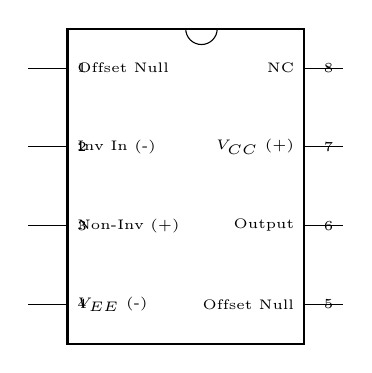
\begin{tikzpicture}
        \draw[thick] (0,0) rectangle (3,4);
        \draw (1.5,4) arc (180:360:0.2);
        \foreach \y in {1,2,3,4} {
            \draw (-0.5, 4.5-\y) -- (0, 4.5-\y) node[right, font=\tiny] {\y};
            \draw (3, 4.5-\y) -- (3.5, 4.5-\y) node[left, font=\tiny] {\the\numexpr9-\y};
        }
        % Labels
        \node[right, font=\tiny] at (0, 3.5) {Offset Null};
        \node[right, font=\tiny] at (0, 2.5) {Inv In (-)};
        \node[right, font=\tiny] at (0, 1.5) {Non-Inv (+)};
        \node[right, font=\tiny] at (0, 0.5) {$V_{EE}$ (-)};
        
        \node[left, font=\tiny] at (3, 3.5) {NC};
        \node[left, font=\tiny] at (3, 2.5) {$V_{CC}$ (+)};
        \node[left, font=\tiny] at (3, 1.5) {Output};
        \node[left, font=\tiny] at (3, 0.5) {Offset Null};
    \end{tikzpicture}
    \end{center}
    
    \textbf{Pin Configuration:}
    \begin{tabulary}{\textwidth}{C|L|L}
        \toprule
        \textbf{Pin} & \textbf{Function} & \textbf{Description} \\
        \midrule
        \textbf{1} & Offset Null & Offset adjustment \\
        \textbf{2} & Inverting Input & Negative input \\
        \textbf{3} & Non-inverting Input & Positive input \\
        \textbf{4} & $-V_{CC}$ & Negative supply \\
        \textbf{5} & Offset Null & Offset adjustment \\
        \textbf{6} & Output & Amplifier output \\
        \textbf{7} & $+V_{CC}$ & Positive supply \\
        \textbf{8} & NC & No connection \\
        \bottomrule
    \end{tabulary}
    
    \begin{mnemonicbox}
        \mnemonic{Null, Negative, Positive, Negative supply, Null, Output, Positive supply, Nothing}
    \end{mnemonicbox}
\end{solutionbox}

% Question 4(b) [4 marks]
\questionmarks{4}{b}{4}
\textbf{Define the following OP-AMP parameters. 1. Input offset voltage 2. CMRR}

\begin{solutionbox}
    \textbf{Answer}:
    These parameters define the non-ideal characteristics of practical operational amplifiers.
    
    \textbf{1. Input Offset Voltage ($V_{io}$):}
    \begin{itemize}
        \item \textbf{Definition}: DC voltage applied between inputs to make output zero
        \item \textbf{Typical value}: 1-5 mV for 741
        \item \textbf{Cause}: Mismatch in input transistors
        \item \textbf{Effect}: Output error in DC applications
    \end{itemize}
    
    \textbf{2. Common Mode Rejection Ratio (CMRR):}
    \begin{itemize}
        \item \textbf{Definition}: Ability to reject common signals at both inputs
        \item \textbf{Formula}: $CMRR = A_d/A_{cm}$
        \item \textbf{Typical value}: 90 dB for 741
        \item \textbf{Importance}: Noise immunity
    \end{itemize}
    
    \begin{tabulary}{\textwidth}{L|L|L|L|L}
        \toprule
        \textbf{Parameter} & \textbf{Symbol} & \textbf{Unit} & \textbf{Ideal} & \textbf{741 Typical} \\
        \midrule
        \textbf{Input Offset Voltage} & $V_{io}$ & mV & 0 & 2 \\
        \textbf{CMRR} & - & dB & $\infty$ & 90 \\
        \bottomrule
    \end{tabulary}
    
    \begin{mnemonicbox}
        \mnemonic{Offset creates Output error, CMRR Rejects common signals}
    \end{mnemonicbox}
\end{solutionbox}

% Question 4(c) [7 marks]
\questionmarks{4}{c}{7}
\textbf{Explain inverting amplifier using IC 741 in detail.}

\begin{solutionbox}
    \textbf{Answer}:
    Inverting amplifier uses negative feedback with input applied to inverting terminal.
    
    \textbf{Circuit Diagram:}
    \begin{center}
    \begin{circuitikz}[american]
        \draw (0,0) node[op amp](opamp){}
        (opamp.+) node[ground]{}
        (opamp.-) to[R, l=$R_1$] (-2, 0.5) node[left]{$V_{in}$}
        (opamp.-) -- (0, 0.5) -- (0, 1.5) to[R, l=$R_f$] (2, 1.5) -- (opamp.out)
        (opamp.out) -- (3,0) node[right]{$V_{out}$};
    \end{circuitikz}
    \end{center}
    
    \textbf{Analysis:}
    Using virtual short concept:
    \begin{itemize}
        \item \textbf{$V_+ = V_- = 0V$} (virtual ground)
        \item \textbf{Input current}: $I_1 = V_{in}/R_1$
        \item \textbf{Feedback current}: $I_f = V_{out}/R_f$
        \item \textbf{Current balance}: $I_1 = I_f$ (no current into op-amp)
    \end{itemize}
    
    \textbf{Derivation:}
    \begin{itemize}
        \item $V_{in}/R_1 = -V_{out}/R_f$
        \item \textbf{Voltage Gain: $A_v = -R_f/R_1$}
    \end{itemize}
    
    \textbf{Characteristics:}
    \begin{tabulary}{\textwidth}{L|L|L}
        \toprule
        \textbf{Parameter} & \textbf{Expression} & \textbf{Notes} \\
        \midrule
        \textbf{Voltage Gain} & $-R_f/R_1$ & Negative sign \\
        \textbf{Input Impedance} & $R_1$ & Low impedance \\
        \textbf{Output Impedance} & $\approx 0\Omega$ & Very low \\
        \textbf{Bandwidth} & $f = GBW/|A_v|$ & Gain-bandwidth product \\
        \bottomrule
    \end{tabulary}
    
    \textbf{Applications:}
    \begin{itemize}
        \item \textbf{Signal inversion}: Phase reversal
        \item \textbf{Scale factor}: Programmable gain
        \item \textbf{AC amplification}: With coupling capacitors
    \end{itemize}
    
    \begin{mnemonicbox}
        \mnemonic{Inverting Input gives Inverted output}
    \end{mnemonicbox}
\end{solutionbox}

% Question 4(a OR) [3 marks]
\questionmarks{4}{a}{3}
\textbf{List characteristics of ideal OP-AMP.}

\begin{solutionbox}
    \textbf{Answer}:
    Ideal op-amp represents perfect amplifier with theoretical limits for all parameters.
    
    \begin{tabulary}{\textwidth}{L|L|L}
        \toprule
        \textbf{Parameter} & \textbf{Ideal Value} & \textbf{Practical Impact} \\
        \midrule
        \textbf{Open Loop Gain} & $\infty$ & Perfect amplification \\
        \textbf{Input Impedance} & $\infty$ & No input current \\
        \textbf{Output Impedance} & $0\Omega$ & Perfect voltage source \\
        \textbf{Bandwidth} & $\infty$ & No frequency limitation \\
        \textbf{CMRR} & $\infty$ & Perfect noise rejection \\
        \textbf{Slew Rate} & $\infty$ & No slew rate limiting \\
        \textbf{Input Offset} & 0V & No DC errors \\
        \bottomrule
    \end{tabulary}
    
    \begin{itemize}
        \item \textbf{Perfect performance}: All parameters optimized
        \item \textbf{Design simplification}: Analysis becomes easier
        \item \textbf{Practical approximation}: Close to ideal in many applications
    \end{itemize}
    
    \begin{mnemonicbox}
        \mnemonic{Infinite Input, Zero Output, Perfect Performance}
    \end{mnemonicbox}
\end{solutionbox}

% Question 4(b OR) [4 marks]
\questionmarks{4}{b}{4}
\textbf{Draw and explain summing amplifier using Op-amp.}

\begin{solutionbox}
    \textbf{Answer}:
    Summing amplifier adds multiple input voltages with programmable gain for each input.
    
    \textbf{Circuit Diagram:}
    \begin{center}
    \begin{circuitikz}[american]
        \draw (0,0) node[op amp](opamp){}
        (opamp.+) node[ground]{}
        (opamp.-) -- (-1, 0.5) 
        (-1, 0.5) to[R, l=$R_1$] (-3, 1.5) node[left]{$V_1$}
        (-1, 0.5) to[R, l=$R_2$] (-3, 0.5) node[left]{$V_2$}
        (-1, 0.5) to[R, l=$R_3$] (-3, -0.5) node[left]{$V_3$}
        (opamp.-) -- (0, 0.5) -- (0, 1.5) to[R, l=$R_f$] (2, 1.5) -- (opamp.out)
        (opamp.out) -- (3,0) node[right]{$V_{out}$};
    \end{circuitikz}
    \end{center}
    
    \textbf{Analysis:}
    Using virtual ground concept ($V_- = 0V$):
    \begin{itemize}
        \item \textbf{Current through R1}: $I_1 = V_1/R_1$
        \item \textbf{Current through R2}: $I_2 = V_2/R_2$
        \item \textbf{Current through R3}: $I_3 = V_3/R_3$
        \item \textbf{Total input current}: $I_{in} = I_1 + I_2 + I_3$
    \end{itemize}
    
    \textbf{Output Equation:}
    \[ V_{out} = -R_f(V_1/R_1 + V_2/R_2 + V_3/R_3) \]
    
    \textbf{Special Cases:}
    \begin{itemize}
        \item \textbf{Equal resistors}: $V_{out} = -(R_f/R)(V_1 + V_2 + V_3)$
        \item \textbf{Unity gain}: $R_f = R$, $V_{out} = -(V_1 + V_2 + V_3)$
    \end{itemize}
    
    \begin{mnemonicbox}
        \mnemonic{Sum inputs, Scale by resistor ratios}
    \end{mnemonicbox}
\end{solutionbox}

% Question 4(c OR) [7 marks]
\questionmarks{4}{c}{7}
\textbf{Explain differential amplifier using IC 741 in detail.}

\begin{solutionbox}
    \textbf{Answer}:
    Differential amplifier amplifies the difference between two input signals while rejecting common signals.
    
    \textbf{Circuit Diagram:}
    \begin{center}
    \begin{circuitikz}[american]
        \draw (0,0) node[op amp](opamp){}
        (opamp.-) to[R, l=$R_1$] (-2, 0.5) node[left]{$V_1$}
        (opamp.+) to[R, l=$R_2$] (-2, -0.5) node[left]{$V_2$}
        (opamp.+) to[R, l=$R_3$] (0, -2) node[ground]{}
        (opamp.-) -- (0, 0.5) -- (0, 1.5) to[R, l=$R_f$] (2, 1.5) -- (opamp.out)
        (opamp.out) -- (3,0) node[right]{$V_{out}$};
    \end{circuitikz}
    \end{center}
    
    \textbf{Analysis:}
    For the non-inverting input:
    \begin{itemize}
        \item $V_+ = V_2 \times \frac{R_3}{R_2+R_3}$
    \end{itemize}
    
    For the inverting input using virtual short:
    \begin{itemize}
        \item $V_- = V_+ = V_2 \times \frac{R_3}{R_2+R_3}$
    \end{itemize}
    
    Using current balance:
    \begin{itemize}
        \item $\frac{V_1-V_-}{R_1} = \frac{V_--V_{out}}{R_f}$
    \end{itemize}
    
    \textbf{Output Equation:}
    When $R_1 = R_2$ and $R_3 = R_f$:
    \[ V_{out} = \frac{R_f}{R_1}(V_2 - V_1) \]
    
    \textbf{Key Features:}
    \begin{tabulary}{\textwidth}{L|L|L}
        \toprule
        \textbf{Parameter} & \textbf{Value} & \textbf{Advantage} \\
        \midrule
        \textbf{Differential Gain} & $R_f/R_1$ & Amplifies difference \\
        \textbf{Common Mode Gain} & $\approx 0$ & Rejects common signals \\
        \textbf{CMRR} & Very high & Excellent noise immunity \\
        \bottomrule
    \end{tabulary}
    
    \begin{mnemonicbox}
        \mnemonic{Difference amplified, Common rejected}
    \end{mnemonicbox}
\end{solutionbox}

% Question 5(a) [3 marks]
\questionmarks{5}{a}{3}
\textbf{Draw the circuit of integrator using Op-amp and its input and output waveforms.}

\begin{solutionbox}
    \textbf{Answer}:
    Op-amp integrator performs mathematical integration of input signal using RC feedback.
    
    \textbf{Circuit Diagram:}
    \begin{center}
    \begin{circuitikz}[american]
        \draw (0,0) node[op amp](opamp){}
        (opamp.-) to[R, l=$R$] (-2, 0.5) node[left]{$V_{in}$}
        (opamp.+) node[ground]{}
        (opamp.-) -- (0, 0.5) -- (0, 1.5) to[C, l=$C$] (2, 1.5) -- (opamp.out)
        (opamp.out) -- (3,0) node[right]{$V_{out}$};
    \end{circuitikz}
    \end{center}
    
    \textbf{Waveforms:}
    \begin{center}
    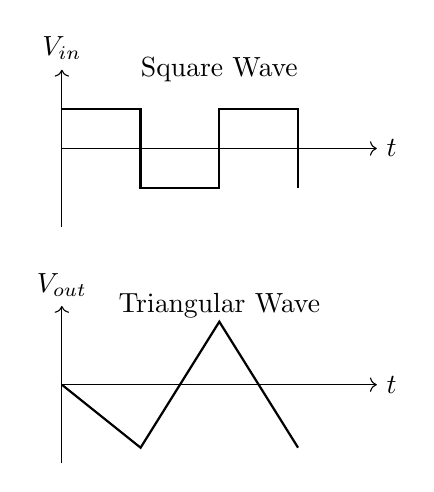
\begin{tikzpicture}
        % Input square wave
        \draw[->] (0,3) -- (4,3) node[right]{$t$};
        \draw[->] (0,2) -- (0,4) node[above]{$V_{in}$};
        \draw[thick] (0,3.5) -- (1,3.5) -- (1,2.5) -- (2,2.5) -- (2,3.5) -- (3,3.5) -- (3,2.5);
        \node at (2,4) {Square Wave};
        
        % Output triangular wave
        \draw[->] (0,0) -- (4,0) node[right]{$t$};
        \draw[->] (0,-1) -- (0,1) node[above]{$V_{out}$};
        \draw[thick] (0,0) -- (1,-0.8) -- (2,0.8) -- (3,-0.8);
        \node at (2,1) {Triangular Wave};
    \end{tikzpicture}
    \end{center}
    
    \textbf{Operation:}
    \begin{itemize}
        \item \textbf{Integration function}: $V_{out} = -\frac{1}{RC}\int V_{in} dt$
        \item \textbf{Square wave input}: Produces triangular output
        \item \textbf{Ramp generation}: Constant input gives linear ramp
    \end{itemize}
    
    \begin{mnemonicbox}
        \mnemonic{Integration creates Triangular from square}
    \end{mnemonicbox}
\end{solutionbox}

% Question 5(b) [4 marks]
\questionmarks{5}{b}{4}
\textbf{State advantage and disadvantage of push-pull arrangement of power amplifier}

\begin{solutionbox}
    \textbf{Answer}:
    Push-pull configuration uses two transistors operating in complementary fashion for power amplification.
    
    \textbf{Advantages:}
    \begin{tabulary}{\textwidth}{L|L|L}
        \toprule
        \textbf{Advantage} & \textbf{Benefit} & \textbf{Application} \\
        \midrule
        \textbf{High Efficiency} & Up to 78.5\% & Battery operated \\
        \textbf{No Transformer} & Compact design & Portable devices \\
        \textbf{Low Distortion} & Better linearity & Audio systems \\
        \textbf{Heat Distribution} & Shared between transistors & Thermal management \\
        \bottomrule
    \end{tabulary}
    
    \textbf{Disadvantages:}
    \begin{tabulary}{\textwidth}{L|L|L}
        \toprule
        \textbf{Disadvantage} & \textbf{Problem} & \textbf{Solution} \\
        \midrule
        \textbf{Crossover Distortion} & Dead zone at zero crossing & Class AB bias \\
        \textbf{Component Matching} & Requires matched transistors & Careful selection \\
        \textbf{Thermal Runaway} & Temperature coefficient mismatch & Thermal coupling \\
        \bottomrule
    \end{tabulary}
    
    \begin{mnemonicbox}
        \mnemonic{Push-Pull Provides Power but Problems exist}
    \end{mnemonicbox}
\end{solutionbox}

% Question 5(c) [7 marks]
\questionmarks{5}{c}{7}
\textbf{Draw and explain astable multivibrator using 555 timer IC.}

\begin{solutionbox}
    \textbf{Answer}:
    Astable multivibrator generates continuous square wave output without external trigger using 555 timer.
    
    \textbf{Circuit Diagram:}
    \begin{center}
    \begin{circuitikz}
        \draw (0,0) node[draw, minimum width=2cm, minimum height=2.5cm] (timer) {555};
        \draw (timer.west) ++(0, 0.5) coordinate (thresh) node[left] {Thresh(6)};
        \draw (timer.west) ++(0, -0.5) coordinate (trig) node[left] {Trig(2)};
        \draw (timer) ++(-0.5, 1.25) coordinate (disch) -- ++(0, 0.5) node[left] {Disch(7)};
        \draw (timer) ++(1, 0) -- ++(1,0) node[right] {Output(3)};
        
        % RC Network
        \draw (disch) ++(0, 1) node[vcc]{$V_{CC}$} to[R, l=$R_A$] (disch);
        \draw (disch) to[R, l=$R_B$] (thresh);
        \draw (thresh) -- (trig); % 2 and 6 connected
        \draw (trig) to[C, l=$C$] ++(0, -1.5) node[ground]{};
        \draw (thresh) -- ++(-1.5, 0) -- ++(0, -3.5) -- ++(1.5, 0) -- (trig); % Connection
    \end{circuitikz}
    \end{center}
    
    \textbf{Operation:}
    \begin{enumerate}
        \item \textbf{Charging phase}: C charges through $R_A + R_B$
        \item \textbf{Threshold reached}: At $2/3 V_{CC}$, output goes LOW
        \item \textbf{Discharging phase}: C discharges through $R_B$
        \item \textbf{Trigger reached}: At $1/3 V_{CC}$, output goes HIGH
        \item \textbf{Cycle repeats}: Continuous oscillation
    \end{enumerate}
    
    \textbf{Timing Equations:}
    \begin{itemize}
        \item \textbf{HIGH time}: $t_1 = 0.693(R_A + R_B)C$
        \item \textbf{LOW time}: $t_2 = 0.693(R_B)C$
        \item \textbf{Total period}: $T = t_1 + t_2 = 0.693(R_A + 2R_B)C$
        \item \textbf{Frequency}: $f = \frac{1.44}{(R_A + 2R_B)C}$
        \item \textbf{Duty cycle}: $D = \frac{R_A + R_B}{R_A + 2R_B} \times 100\%$
    \end{itemize}
    
    \begin{mnemonicbox}
        \mnemonic{Astable Always oscillates Automatically}
    \end{mnemonicbox}
\end{solutionbox}

% Question 5(a OR) [3 marks]
\questionmarks{5}{a}{3}
\textbf{Draw the block diagram of Op-amp and explain it.}

\begin{solutionbox}
    \textbf{Answer}:
    Op-amp internal structure consists of multiple stages for high gain and performance.
    
    \textbf{Block Diagram:}
    \begin{center}
    \begin{tikzpicture}[node distance=2.5cm, auto, >=latex]
        \node [gtu input] (in) {Inputs};
        \node [gtu block, right of=in] (diff) {Differential\\Amplifier};
        \node [gtu block, right of=diff] (gain) {Intermediate\\Amplifier};
        \node [gtu block, right of=gain] (level) {Level\\Shifter};
        \node [gtu block, right of=level] (outstage) {Output\\Stage};
        \node [right of=outstage, node distance=2cm] (out) {Output};
        
        \draw [gtu arrow] (in) -- (diff);
        \draw [gtu arrow] (diff) -- (gain);
        \draw [gtu arrow] (gain) -- (level);
        \draw [gtu arrow] (level) -- (outstage);
        \draw [gtu arrow] (outstage) -- (out);
    \end{tikzpicture}
    \end{center}
    
    \textbf{Stage Functions:}
    \begin{tabulary}{\textwidth}{L|L|L}
        \toprule
        \textbf{Stage} & \textbf{Function} & \textbf{Characteristics} \\
        \midrule
        \textbf{Differential Input} & High input impedance & Low offset, high CMRR \\
        \textbf{Intermediate Amplifier} & High voltage gain & Most of the gain \\
        \textbf{Level Shifter} & DC level adjustment & Couples AC stages \\
        \textbf{Output Stage} & Low output impedance & Current buffer \\
        \bottomrule
    \end{tabulary}
    
    \begin{mnemonicbox}
        \mnemonic{Differential Input, Intermediate gain, Level shift, Output buffer}
    \end{mnemonicbox}
\end{solutionbox}

% Question 5(b OR) [4 marks]
\questionmarks{5}{b}{4}
\textbf{Explain about the terms related to power amplifier. i) Efficiency ii) Distortion.}

\begin{solutionbox}
    \textbf{Answer}:
    These parameters determine power amplifier performance and suitability for applications.
    
    \textbf{i) Efficiency ($\eta$):}
    \begin{itemize}
        \item \textbf{Definition}: Ratio of AC output power to DC input power
        \item \textbf{Formula}: $\eta = P_o(AC)/P_{in}(DC) \times 100\%$
        \item \textbf{Importance}: Determines heat dissipation and battery life
    \end{itemize}
    
    \begin{tabulary}{\textwidth}{L|L|L}
        \toprule
        \textbf{Class} & \textbf{Efficiency} & \textbf{Application} \\
        \midrule
        \textbf{A} & 25\% & Low power, high fidelity \\
        \textbf{B} & 78.5\% & Push-pull amplifiers \\
        \textbf{AB} & 60-70\% & Audio amplifiers \\
        \textbf{C} & >90\% & RF applications \\
        \bottomrule
    \end{tabulary}
    
    \textbf{ii) Distortion:}
    \begin{itemize}
        \item \textbf{Definition}: Unwanted changes in output signal shape
        \item \textbf{Types}: Harmonic, intermodulation, crossover
        \item \textbf{Measurement}: Total Harmonic Distortion (THD)
    \end{itemize}
    
    \begin{mnemonicbox}
        \mnemonic{Efficiency measures Energy use, Distortion shows signal Degradation}
    \end{mnemonicbox}
\end{solutionbox}

% Question 5(c OR) [7 marks]
\questionmarks{5}{c}{7}
\textbf{Draw pin diagram of 555 timer IC. Also draw circuit diagram of two stage sequential timer using 555 timer IC.}

\begin{solutionbox}
    \textbf{Answer}:
    555 timer is versatile IC used for timing applications with standard 8-pin package.
    
    \textbf{Pin Diagram:}
    \begin{center}
    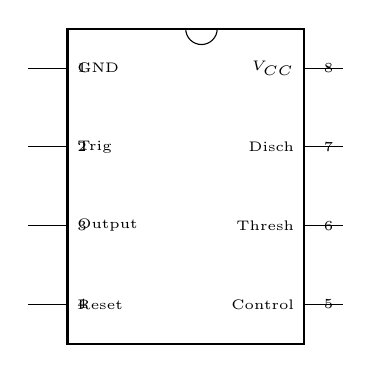
\begin{tikzpicture}
        \draw[thick] (0,0) rectangle (3,4);
        \draw (1.5,4) arc (180:360:0.2);
        \foreach \y in {1,2,3,4} {
            \draw (-0.5, 4.5-\y) -- (0, 4.5-\y) node[right, font=\tiny] {\y};
            \draw (3, 4.5-\y) -- (3.5, 4.5-\y) node[left, font=\tiny] {\the\numexpr9-\y};
        }
        % Labels
        \node[right, font=\tiny] at (0, 3.5) {GND};
        \node[right, font=\tiny] at (0, 2.5) {Trig};
        \node[right, font=\tiny] at (0, 1.5) {Output};
        \node[right, font=\tiny] at (0, 0.5) {Reset};
        
        \node[left, font=\tiny] at (3, 3.5) {$V_{CC}$};
        \node[left, font=\tiny] at (3, 2.5) {Disch};
        \node[left, font=\tiny] at (3, 1.5) {Thresh};
        \node[left, font=\tiny] at (3, 0.5) {Control};
    \end{tikzpicture}
    \end{center}
    
    \textbf{Two Stage Sequential Timer Circuit:}
    \begin{center}
    \begin{circuitikz}
        % Stage 1
        \draw (0,4) node[draw, minimum width=1.5cm, minimum height=2cm] (IC1) {555A};
        \draw (IC1) ++(-2, 1) node[vcc]{$V_{CC}$} to[R, l=$R_2$] ++(0, -1) -- ++(1, 0); % connect to 7
        \draw (IC1) ++(-2, 0) -- ++(1,0); 
        \draw (IC1.west) ++(0, -0.5) to[C, l=$C_1$] ++(0, -1.5) node[ground]{};
        
        % Stage 2
        \draw (5,4) node[draw, minimum width=1.5cm, minimum height=2cm] (IC2) {555B};
        
        % Connection
        \draw (IC1.east) -- ++(1,0) -- (IC2.west);
        
        % Simplified block diagram style for sequential timer
    \end{circuitikz}
    \end{center}
    
    \textbf{Operation:}
    \begin{enumerate}
        \item \textbf{First timer}: Operates in monostable mode
        \item \textbf{Trigger applied}: First timer gives output pulse
        \item \textbf{Output duration}: $T_1 = 1.1 \times R_2 \times C_1$
        \item \textbf{Second timer}: Triggered by first timer's output
        \item \textbf{Sequential operation}: Second timer starts after first completes
        \item \textbf{Total delay}: $T_1 + T_2$ where $T_2 = 1.1 \times R_4 \times C_2$
    \end{enumerate}
    
    \begin{mnemonicbox}
        \mnemonic{Sequential Stages Start Separately}
    \end{mnemonicbox}
\end{solutionbox}

\end{document}
